\chapter{Fundamentos Teóricos}
En este capítulo se describirán aquellos conceptos teóricos fundamentales para comprender el trabajo realizado en este proyecto.

\section{Optimización}
La optimización es un campo de estudio que trata, mediante el uso de las adecuadas herramientas matemáticas, de maximizar o minimizar una función objetivo. Esto significa, obtener la mejor solución posible para un problema dado dentro de un conjunto de alternativas y normalmente sujeto a una serie de restricciones que hacen de una solución satisfacible. Es un área interdisciplinar que aborda desde campos tales como la Economía, Ingeniería, Biología y muchas otras tantas disciplinas.\\[6pt]
La optimización es una disciplina arraigada en la naturaleza humana. Este impulso innato hacia la optimización ha llevado al desarrollo de diversas metodologías y técnicas a lo largo de la historia, desde los rudimentarios métodos de prueba y error hasta los sofisticados algoritmos de optimización computacional utilizados en la actualidad.

\subsection{Definición general de un problema de optimización}
Para poder convertir un problema abstracto en un problema de optimización concreto, con el que se pueda trabajar, es necesario establecer ciertos elementos fundamentales que lo definan de manera precisa y clara. En general, un problema de optimización se expresa de la siguiente forma~\cite{inbook}:

\begin{subequations}
    \begin{alignat}{2}
         & \text{Función objetivo a minimizar}                       & \qquad & f(x)\label{eq:optProb}                             \\
         & \text{Sujeto a} \nonumber                                                                                               \\
         & s \text{ restricciones de desigualdad}                    & \qquad & g_i(x)\leq 0, \quad j=1,2,...,s\label{eq:optProb2} \\
         & w \text{ restricciones de igualdad}                       & \qquad & h_j(x) = 0, \quad j=1,2,...,w\label{eq:optProb3}   \\
         & \text{Donde el número de variables es dado por} \nonumber & \qquad & x_i, \quad i=1,2,...,n
    \end{alignat}
\end{subequations}

La definición general de un problema de optimización proporciona una estructura sólida para abordar el problema abstracto. Establece la función objetivo que se busca minimizar o maximizar, junto con las restricciones que deben cumplirse. Estas restricciones pueden ser tanto desigualdades como igualdades, y todas juntas definen el \textbf{espacio de búsqueda} del problema.

\subsection{Función objetivo y función fitness}
Ambos términos, aunque a menudo se utilizan como sinónimos, desempeñan roles distintos en el ámbito de la optimización. La función \textit{objetivo}, como su nombre indica, establece el objetivo a alcanzar en la resolución del problema. Esta función cuantifica el rendimiento de las soluciones encontradas en relación con el objetivo específico del problema, que puede ser maximizar ganancias, minimizar distancia, entre otros objetivos. Por otro lado, la función de \textit{fitness}  evalúa la idoneidad de una solución dentro de una población de soluciones. Es decir, determina la calidad relativa de la solución respecto a otras alternativas.

Debe destacarse que la métrica de la función de \textit{fitness} suele ser estrictamente positiva, ya que representa la calidad de una solución, generalmente en un rango de valores entre $0$ y $1$. Por otro lado, la función objetivo puede ser positiva o negativa, dependiendo de si se busca maximizar o minimizar el objetivo. Además, la función de aptitud también puede llegar a ser una aproximación de la función objetivo, pero no necesariamente coinciden exactamente.\\[6pt]
Resumiendo, podría decirse que la función \textit{fitness} es un tipo particular de función objetivo que se utiliza como métrica de rendimiento~\cite{eiben2015}.

\subsection{Puntos globales o locales}
Se conocen como punto de óptimo global (mínimo o máximo) la solución (o vector hablando en términos matemáticos) cuyo valor para la función objetivo es el más grande en todo el espacio de soluciones posible, es decir, el espacio de búsqueda. Los puntos locales en cambio son varios, no solo uno como es el global. Son soluciones máximas o mínimas dentro de una región de soluciones.

\begin{figure}[H]
    \begin{center}
        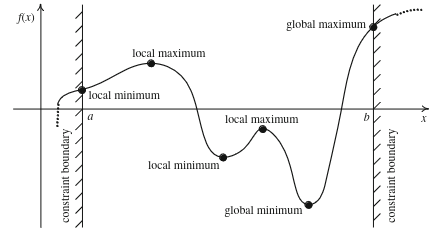
\includegraphics[width=1.2\textwidth]{imagenes/min-max_points.png}
    \end{center}
    \caption{En esta figura extraida de \cite{inbook} puede observarse de manera intuitiva la diferencia entre punto global y puntos locales. El máximo global es el valor más alto para $f(x)$ en el espacio, mientras que un máximo global solo representa el valor más alto dentro de un ``vecindario"}
\end{figure}

Sea $f(x)$ una función a maximizar y $x^*$ una solución óptima. Un objetivo $G(x)$ está en su máximo global sí y solo si~\cite{inbook}:
\begin{equation}
    f(x^*) \geq f(x) \quad \forall x
\end{equation}
En cambio el objetivo está en un máximo local en el punto $x^*$ si:
\begin{equation}
    \begin{split}
        f(x^*) \geq f(x) \quad & \forall x \\
        & \text{dentro de un vecindario de } x^*\text{~\cite{inbook}}
    \end{split}
\end{equation}